

\subsection{Ableitungen}

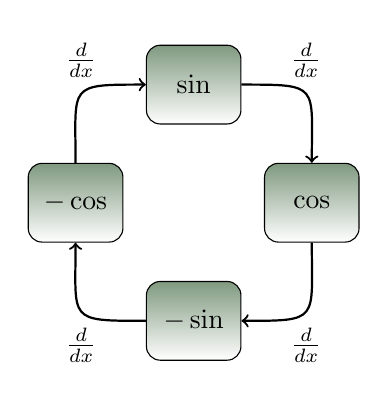
\begin{tikzpicture}
	[	inner sep = 2mm,
		sin/.style={rectangle,minimum width=1.2cm,minimum height=1cm,rounded corners=5pt,draw=black,top color=green!20!black!50},
		abl/.style={rectangle}
	]
	\node at (1.5,0) (sin1) [sin] {$\sin$};
	\node at (0,-1.5) (cos2) [sin] {$-\cos$};
	\node at (1.5,-3) (sin2) [sin] {$-\sin$};
	\node at (3,-1.5) (cos1) [sin] {$\cos$};
	
	\draw[thick,black,->] (sin1.east) .. controls +(right:1cm) and +(up:1cm) ..  (cos1.north)
	node [pos=0.5,above](abl) {$\frac{d}{dx}$};
	\draw[thick,black,->] (cos1.south) .. controls +(down:1cm) and +(right:1cm) .. (sin2.east)
	node [pos=0.5,below](abl) {$\frac{d}{dx}$};
	\draw[thick,black,->] (sin2.west) .. controls +(left:1cm) and +(down:1cm) .. (cos2.south)
	node [pos=0.5,below](abl) {$\frac{d}{dx}$};
	\draw[thick,black,->] (cos2.north) .. controls +(up:1cm) and +(left:1cm) .. (sin1.west)
	node [pos=0.5,above](abl) {$\frac{d}{dx}$};
\end{tikzpicture}